%% This is file `elsarticle-template-1-num.tex',
%%
%% Copyright 2009 Elsevier Ltd
%%
%% This file is part of the 'Elsarticle Bundle'.
%% ---------------------------------------------
%%
%% It may be distributed under the conditions of the LaTeX Project Public
%% License, either version 1.2 of this license or (at your option) any
%% later version.  The latest version of this license is in
%%    http://www.latex-project.org/lppl.txt
%% and version 1.2 or later is part of all distributions of LaTeX
%% version 1999/12/01 or later.
%%
%% The list of all files belonging to the 'Elsarticle Bundle' is
%% given in the file `manifest.txt'.
%%
%% Template article for Elsevier's document class `elsarticle'
%% with numbered style bibliographic references
%%
%% $Id: elsarticle-template-1-num.tex 149 2009-10-08 05:01:15Z rishi $
%% $URL: http://lenova.river-valley.com/svn/elsbst/trunk/elsarticle-template-1-num.tex $
%%

%\documentclass[preprint,authoryear,review,12pt]{elsarticle}
\documentclass[final,5p,times,twocolumn]{elsarticle}

%% Use the option review to obtain double line spacing
%% \documentclass[preprint,review,12pt]{elsarticle}

%% Use the options 1p,two column; 3p; 3p,twocolumn; 5p; or 5p,twocolumn
%% for a journal layout:
%% \documentclass[final,1p,times]{elsarticle}
%% \documentclass[final,1p,times,twocolumn]{elsarticle}
%% \documentclass[final,3p,times]{elsarticle}
%% \documentclass[final,3p,times,twocolumn]{elsarticle}
%% \documentclass[final,5p,times]{elsarticle}
%% \documentclass[final,5p,times,twocolumn]{elsarticle}


\usepackage{color}
\usepackage{multirow,booktabs,ctable,array}
\usepackage{lscape}
\usepackage{amsmath}
\usepackage{lineno}
\usepackage{ulem}
\usepackage{setspace}
\usepackage{listings}
\usepackage{float}
\usepackage{listings}
\usepackage{color,colortbl}
\usepackage{rccol}
\usepackage[table]{xcolor}

    \definecolor{listcomment}{rgb}{0.0,0.5,0.0}
    \definecolor{listkeyword}{rgb}{0.0,0.0,0.5}
    \definecolor{listnumbers}{gray}{0.65}
    \definecolor{listlightgray}{gray}{0.955}
    \definecolor{listwhite}{gray}{1.0}
    \definecolor{lightcyan}{rgb}{0.88,1,1}

\newcommand{\lstsetcpplong}
{
\lstset{frame = tb,
        framerule = 0.25pt,
        float,
        fontadjust,
        backgroundcolor={\color{listlightgray}},
        basicstyle = {\ttfamily\scriptsize},
        keywordstyle = {\ttfamily\color{listkeyword}\textbf},
        identifierstyle = {\ttfamily},
        commentstyle = {\ttfamily\color{listcomment}\textit},
        stringstyle = {\ttfamily},
        showstringspaces = false,
        showtabs = false,
        numbers = none,
        numbersep = 6pt,
        numberstyle={\ttfamily\color{listnumbers}},
        tabsize = 2,
        language=,
        floatplacement=!h,
        caption={\small \baselineskip 12pt DiReCT long command line menu which is invoked using the `{\ttfamily {-}{-}help}' option.  The short command line menu is obtained by typing `{\ttfamily {-}h}'},
        captionpos=b,
        label=listing:long
        }
}

\floatstyle{plain}
\newfloat{command}{thp}{lop}
\floatname{command}{Command}

%\usepackage[nomarkers,notablist]{endfloat}

%% if you use PostScript figures in your article
%% use the graphics package for simple commands
%% \usepackage{graphics}
%% or use the graphicx package for more complicated commands
%% \usepackage{graphicx}
%% or use the epsfig package if you prefer to use the old commands
%% \usepackage{epsfig}

%% The amssymb package provides various useful mathematical symbols
\usepackage{amssymb}
%% The amsthm package provides extended theorem environments
% \usepackage{amsthm}
 
 \usepackage{makecell}

%% The lineno packages adds line numbers. Start line numbering with
%% \begin{linenumbers}, end it with \end{linenumbers}. Or switch it on
%% for the whole article with \linenumbers after \end{frontmatter}.
%% \usepackage{lineno}

%% natbib.sty is loaded by default. However, natbib options can be
%% provided with \biboptions{...} command. Following options are
%% valid:

%%   round  -  round parentheses are used (default)
%%   square -  square brackets are used   [option]
%%   curly  -  curly braces are used      {option}
%%   angle  -  angle brackets are used    <option>
%%   semicolon  -  multiple citations separated by semi-colon
%%   colon  - same as semicolon, an earlier confusion
%%   comma  -  separated by comma
%%   numbers-  selects numerical citations
%%   super  -  numerical citations as superscripts
%%   sort   -  sorts multiple citations according to order in ref. list
%%   sort&compress   -  like sort, but also compresses numerical citations
%%   compress - compresses without sorting
%%
%% \biboptions{comma,round}

% \biboptions{}

\providecommand{\OO}[1]{\operatorname{O}\bigl(#1\bigr)}

\graphicspath{
             {./Figures/}
             }

\long\def\symbolfootnote[#1]#2{\begingroup%
\def\thefootnote{\fnsymbol{footnote}}\footnote[#1]{#2}\endgroup}



\journal{NeuroImage}

\begin{document}


\begin{frontmatter}

\title{Tilting at Algorithmic Windmills}

\author[label1]{Nicholas J.~Tustison
  \fnref{label0}}
  \fntext[label0]{\scriptsize Corresponding author:  PO Box 801339, Charlottesville, VA 22908; T:  434-924-7730; email address:  ntustison@virginia.edu.
  }
\author[label2]{Brian B.~Avants (combined first author, second author or senior author?)}
\address[label1]{Department of Radiology and Medical Imaging, University of Virginia, Charlottesville, VA}
\address[label2]{Penn Image Computing and Science Laboratory, University of Pennsylvania,
                Philadelphia, PA}

%\maketitle

\linenumbers

\begin{abstract} 
Exploration of neuroscience hypotheses have been greatly enhanced
by the increased availability of high-performance computational resources, large-scale
communal efforts such as the Insight Toolkit and the R statistical project and
algorithmic advancements for data transformations and processing. 
An integral component of the vetting process for novel algorithmic techniques
includes comparison with other methods previously
established within the community.  Public availability, including 
open source distribution, of established packages has significantly 
facilitated these comparative evaluations.  However, complementing the
recent set of papers pointing to serious methodological and statistical
bias considerations in neuroimaging research, we point out potential 
issues associated with a type of measurement bias in comparative algorithmic
evaluations and propose a set of guidelines for authors and reviewers
to minimize this confound.
\end{abstract}
\begin{keyword}
open science \sep reproducibility 
%% keywords here, in the form: keyword \sep keyword
\end{keyword}

\end{frontmatter}
%
%
\newpage

%% MSC codes here, in the form: \MSC code \sep code
%% or \MSC[2008] code \sep code (2000 is the default)

%%
%% Start line numbering here if you want
%%
% \linenumbers

%% The Appendices part is started with the command \appendix;
%% appendix sections are then done as normal sections
%% \appendix

%% \section{}
%% \label{}

%% References
%%
%% Following citation commands can be used in the body text:
%% Usage of \cite is as follows:
%%   \citep{key}          ==>>  [#]
%%   \cite[chap. 2]{key} ==>>  [#, chap. 2]
%%   \citet{key}         ==>>  Author [#]

%% main text

%\section{Introduction}

% Neuroscientific investigations into cortical morphological
% changes/differences have illuminated interesting correlations with
% normal and pathological neurodevelopment in  addition to cognitive function.
Historically rooted in the meticulous work of von Economo \citep{economo2008},
imaging-based structural analysis of the brain plays a fundamental role
in identifying the relationship between cortical morphology, disease and cognition.
Quantitative cortical measures have been demonstrated in conditional 
abnormalities such as 
Huntington's disease \citep{rosas2002,rosas2005,selemon2004}, 
schizophrenia \citep{nesvag2008}, bipolar disorder \cite{lyoo2006}, Alzheimer's disease and frontotemporal
dementia \citep{du2007,dickerson2009}, Parkinson's disease \citep{jubault2011}, Williams syndrome \cite{thompson2005},
multiple sclerosis \citep{ramasamy2009}, autism \citep{chung2005,hardan2006},
migraines \citep{dasilva2007}, chronic smoking \citep{kuhn2010}, alcoholism \citep{fortier2011},
cocaine addiction \citep{makris2008}, Tourette syndrome in children \citep{sowell2008},
scoliosis in
female adolescents \citep{wang2012}, obsessive compulsive
disorder \citep{shin2007}, ADHD \citep{almeida-montes2012}, obesity \citep{raji2010}, and heritable \citep{peterson2009}
and elderly \citep{ballmaier2004} depression.  Cortical thickness also
varies normally as a function of age \citep{kochunov2011},
gender \citep{luders2006a}, untreated transsexuality \citep{zubiaurre-elorza2012},  handedness
\citep{luders2006,amunts2007}, intelligence \citep{shaw2006}, athletic
ability \citep{wei2011}, musical ability \citep{bermudez2009,foster2010}, 
tendency toward criminality \citep{raine2011}, and Tetris-playing
ability in female adolescents \citep{haier2009}.  Additionally,
recent studies demonstrate possible functional 
connectivity relationships using cortical thickness measures
\cite{worsley2005,lerch2006,he2007}.
Although these findings
are subject to debate and interpretation \citep{gernsbacher2007}, 
the availability of quantitative
computational methods for extracting such information
has proven invaluable for developing and refining fundamental 
neuroscience hypotheses.

Computational methods for analyzing the cortex may be 
broadly characterized as surface mesh-based or volumetric \citep{scott2009,clarkson2011}.  Representative of the former is the
Freesurfer%
\footnote{
http://surfer.nmr.mgh.harvard.edu/
}
cortical modeling software package \citep{dale1999,fischl1999,fischl2000,fischl2002,fischl2004}
which owes its popularity to public availability, excellent documentation, 
good performance, and  integration with other toolkits, such as the extensive FMRIB software 
library (FSL) \citep{smith2004}.  Similar to other surface
approaches (e.g. \cite{davatzikos1996,magnotta1999,macdonald2000,kim2005}), the pial
and white matter surfaces from individual subject MR data are modeled with polygonal meshes  
which are then used to determine local cortical thickness based on a specified correspondence between 
the surface models.

Image volumetric (or meshless) techniques vary both in algorithmic terms as well as
the underlying definition of cortical thickness.  An early, foundational technique is the 
method of \cite{jones2000} in which the inner and outer surface geometry is used to determine the
solution to Laplace's equation where thickness is measured by integrating along the 
tangents of the resulting field lines spanning the boundary surfaces.  Subsequent contributions
improved upon the original formulation.  For example, in \cite{yezzi2003}, an Eulerian PDE approach
was proposed to facilitate the computation of correspondence paths.  Extending the surface-based
work of \cite{macdonald2000}, the hybrid approach of
\cite{kim2005} uses the discrete Laplacian field to deform the white matter surface mesh towards the 
pial surface.    Although the Laplacian-based approach has several advantages
including generally lower computational times and 
non-crossing correspondence paths, direct correlative assessments with histology
are potentially problematic as the quantified distances 
are not necessarily Euclidean.  Other volumetric algorithms employ coupled
level sets \citep{zeng1999}, model-free intelligent search strategies either normal to 
the gray-white matter interface \citep{scott2009} or using a min-max rule \citep{clement-vachet2011}.
Most relevant to this work is the DiReCT (Diffeomorphic Registration-based 
Cortical Thickness) algorithm proposed in \cite{das2009} where generated
diffeomorphic mappings between the 
white and pial matter surfaces are used to propagate thickness values 
through the cortical gray matter.  A unique benefit of DiReCT is that it
naturally estimates the boundaries of buried sulci by employing a
diffeomorphic constraint on the probabilistic estimate of the gray
matter and cerebrospinal fluid interface.  

Despite the variety of techniques for estimating cortical thickness
from imaging data (of which
only a fraction are cited), several common preprocessing components
may be identified.
The most fundamental of these include inhomogeneity correction, skull stripping, and $n$-tissue segmentation 
for differentiating the gray and white matter.  For statistical analysis 
across large populations, construction of population-specific unbiased templates
is also potentially beneficial \cite{evans2012}.
In addition, intermediate steps might include a crucial registration component, e.g. 
propagating template-based tissue priors for improved segmentation.

  The requisite
additional components apart from the actual cortical thickness estimation, 
coupled with the general lack of availability of published
algorithms \cite{kovacevic2006}, inhibits performing studies by external researchers 
and makes comparative evaluations difficult.  For example, one recent evaluation 
study \citep{clarkson2011} compared
Freesurfer (a surface-based method) with two volumetric methods \citep{jones2000,das2009}.
Whereas the entire Freesurfer processing pipeline has been made publicly available, 
tuned by the original authors in terms of implementation, and described in great detail 
(specifically in terms of suggested parameters); both volumetric methods were 
implemented solely by the authors of the evaluation (not the actual algorithmic developers) using 
unspecified parameters making the comparisons less than
ideal. Further complicating comparisons is distinct processing domains between
volumetric and surface-based techniques and the potential for the introduction
of bias \cite{klein2010}.

In this work, we describe our Insight Toolkit (ITK)-based cortical thickness pipeline
which is freely available as part of the Advanced Normalization Tools
(ANTs) software package.  This includes all the necessary preprocessing steps consisting
of well-vetted previously published algorithms for bias correction \cite{tustison2010},
brain extraction \cite{avants2010a}, $n$-tissue segmentation \cite{avants2011a},
template construction \cite{avants2010}, and image normalization \cite{avants2011}.
We also describe improvements made to the original DiReCT algorithm \cite{das2009}.
Equally as important, we provide explicit coordination between
these pipeline components complete with a set of useful parameters
which are employed to analyze the publicly available IXI data set. The
full pipeline and parameter set is 
encapsulated in a well-documented shell script which is also available in ANTs. 
Furthermore, we provide all the derived image data and other processing scripts on 
the NITRC repository specifically meant for this publication.  The
availability of both the code and data permits
the set of results described in this work to be fully reproducible.  This
permits other researchers to contrast their own results against
this baseline processing and to adapt the given volumetric pipeline for measuring
cortical thickness with their own datasets.








%This might explain why there have been few evaluation studies.  For example, in
%comparing volumetric and surface-based methods, \cite{clarkson2011} use the
%Freesurfer implementation but rely on their own implementations of published 
%literature which might not be an unbiased evaluation particularly given the 
%complexity of the underlying registration algorithmic work in \cite{das2009}.
%Based solely on the number of citations in the literature,
%the Freesurfer%
%\footnote{
%http://surfer.nmr.mgh.harvard.edu/
%} 
%cortical modeling software package is perhaps the most ubiquitous 
%with several publications detailing various stages of development and
%methodology \citep{dale1999,fischl1999,fischl2000,fischl2002,fischl2004}.  
%Public availability, excellent documentation, good performance, and 
%integration with other toolkits, such as the extensive FMRIB software 
%library (FSL) \cite{smith2004},
%have contributed to its popularity.  



%Freesurfer's individual brain processing pipeline begins with segmentation
%and surface modeling of the gray white matter interface.  Gradients 


%\begin{table*}
%\caption{Component-wise breakdown of reported cortical thickness methods reported in the literature.}
%\begin{tabular*}{0.95\textwidth}{@{\extracolsep{\fill}} c c c c c p{4.5cm} }
%\hline
%{\bf Algorithm} & {\bf V/S} & {\bf Bias correction} & {\bf Brain extraction} & {\bf Segmentation} & \multicolumn{1}{c}{\bf Additional notes} \\
%\hline
%BRAINSURF \cite{magnotta1999} & S & {} & none & Discriminate analysis \cite{harris1999} & {} \\
%ASP \cite{macdonald2000} & S & {} & N3$^\dagger$ \cite{Sled1998} & Neural-nets \cite{ozkan1993} & {}\\
%Laplace \cite{Jones2000} & V & {} & none & simple thresholding & {} \\
%CLASP \cite{kim2005} & V/S & {} & N3$^\dagger$ \cite{Sled1998} & K-NN \cite{cocosco2003} & { Partial volume classification of GM/CSF \cite{Choi1991} is used to facilitate reconstructing the pial surface. }\\
%\cite{hutton2005} & V & {} & {} & {} & {} \\
%DiReCT \cite{das2009} & V & {} & none & FAST$^\dagger$ \cite{zhang2001} & {} \\
%\cite{scott2009} & V & {} & none & E-M Bayes \cite{pokric2001}  & {} \\
%\cite{acosta2009} & V & {} & \cite{van-leemput1999a} & E-M Bayes. \cite{van-leemput1999} & {}\\
%\cite{lerch2005}$^{BrainVisa}$ & {} & {} & {} & {} & {} \\
%CRUISE\cite{han2004,tosun2006} & S& {}  & TOADS$^\dagger$ \cite{bazin2007} & {} \\
%
%CLADA\cite{nakamura2011} & S& {}  & PABIC$^\dagger$ \cite{styner2000} & \cite{nakamura2009} & {longitudinal analysis}\\
%%SIENA$^\dagger$\cite{smith2002} & {} & {} & FAST$^\dagger$ \cite{zhang2001} & {longitudinal analysis}\\
%\hline
%\end{tabular*}
%\end{table*}
%
%Open source packages:
%\begin{itemize}
%\item (http://www.ncbi.nlm.nih.gov/pubmed/15957597) TINA - be sure to read the reviews which aren't very good.
%\item (http://www.nitrc.org/projects/arctic/ %http://www.na-mic.org/Wiki/index.php/UNC_ARCTIC_Tutorial) 
%ARCTIC (Automatic Regional Cortical ThICkness)
%\item Brain Voyager (Goebel?)
%\item TOADS-CRUISE (Tosun et al.) http://www.nitrc.org/projects/toads-cruise/
%\item GAMBIT
%\item http://www.bic.mni.mcgill.ca/thickness\_population\_simulation/ \cite{lerch2005}
%\item Be sure to email Vincent Magnotta to see if they have open source tools in Brains for estimation of cortical thickness
%\end{itemize}

%
%\section{Methods and Materials}

\subsection{ANTs volumetric-based cortical thickness estimation pipeline}

The ANTs-based cortical thickness estimation workflow is illustrated 
in Figure \ref{fig:pipeline}.  The steps are as follows:
\begin{enumerate}
  \item initial N4 bias correction on input anatomical MRI,
  \item brain extraction using a hybrid segmentation/template-based strategy,
  \item alternating between prior-based segmentation and white matter posterior
        probability weighted bias correction,
  \item DiReCT-based cortical thickness estimation, and
  \item optional normalization to specified template.
\end{enumerate}
Each component, including both software and data, is briefly detailed 
below with the relevant references for additional information. 


%We also note that each component is publicly available with all ANTs 
%algorithms available as open source.%
%\footnote{
%http://www.picsl.upenn.edu/ANTS
%}
Additionally, the coordination of all the algorithmic components is
encapsulated in the shell script \verb#antsCorticalThickness.sh#.  This includes
optimal parameters for each of the algorithmic components which has worked
well for our processing and which are used to acquire the results 
described in this work.

%\lstset{frame = tb,
%        framerule = 0.25pt,
%        float,
%        fontadjust,
%        backgroundcolor={\color{listlightgray}},
%        basicstyle = {\ttfamily\scriptsize},
%        keywordstyle = {\ttfamily\color{listkeyword}\textbf},
%        identifierstyle = {\ttfamily},
%        commentstyle = {\ttfamily\color{listcomment}\textit},
%        stringstyle = {\ttfamily},
%        showstringspaces = false,
%        showtabs = false,
%        numbers = none,
%        numbersep = 6pt,
%        numberstyle={\ttfamily\color{listnumbers}},
%        tabsize = 2,
%        language=,
%        floatplacement=!h,
%        caption={\small \baselineskip 12pt DiReCT long command line menu which is invoked using the `{\ttfamily {-}{-}help}' option.  The short command line menu is obtained by typing `{\ttfamily {-}h}'}.,
%        captionpos=b,
%        label=listing:long
%        }
%\lstsetcpplong
%\begin{lstlisting}
%This script, apb.sh, performs T1 anatomical brain 
%processing where the following steps are currently 
%applied:
%
%  1. Brain extraction
%  2. Brain 3-tissue segmentation
%  3. Cortical thickness
%  4. (Optional) registration to a template
%
%Usage:
%
%abp.sh -d ImageDimension
%       -i T1Image.nii.gz
%       -e BrainExtractionTemplate
%       -m BrainExtractionProbabilityMask
%       -l BrainParcellationTemplate
%       -p BrainParcellationProbabilityMask
%       <OPTARGS>
%       -o OutputPrefix
%
%Example:
%
%abp.sh -d 3 
%       -i t1.nii.gz 
%       -e brainWithSkullTemplate.nii.gz 
%       -m brainPrior.nii.gz 
%       -l corticalLabels.nii.gz 
%       -p corticalLabelPriors.nii.gz 
%       -o output
%
%Compulsory arguments:
%
%     -d:  ImageDimension                        2 or 3 (for 2 or 3 dimensional single image)
%     -a:  Anatomical T1 image                   typically T1.
%     -e:  Brain extraction template             Anatomical template created using e.g. LPBA40 data set with
%                                                buildtemplateparallel.sh in ANTs.
%     -m:  Brain extraction probability mask     Brain probability mask created using e.g. LPBA40 data set which
%                                                have brain masks defined, and warped to anatomical template and
%                                                averaged resulting in a probability image.
%     -l   Brain segmentation template           Anatomical template for brain segmentation.  E.g. NIREP template
%                                                with labels.
%     -p   Brain segmentationpriors              Label probability priors corresponding to the image specified
%                                                with the -l option.  Specified using c-style formatting, e.g.
%                                                -p labelsPriors\%02d.nii.gz.
%     -o:  OutputPrefix                          The following images are created using the specified prefix:
%                                                  * /Users/ntustison/Data//tmp13243//tmpN4Corrected.nii.gz
%                                                  * /Users/ntustison/Data//tmp13243//tmpExtractedBrain.nii.gz
%                                                  * /Users/ntustison/Data//tmp13243//tmp3TissueBrainSegmentation.nii.gz
%                                                  * /Users/ntustison/Data//tmp13243//tmpCorticalThickness.nii.gz
%                                                  * /Users/ntustison/Data//tmp13243//tmpSurfaceCurvature.nii.gz
%
%Optional arguments:
%
%     -s:  image file suffix                     Any of the standard ITK IO formats e.g. nrrd, nii.gz (default), mhd
%     -t:  template for t1 registration
%     -k:  keep temporary files                  Keep brain extraction/segmentation warps, etc (default = false).
%     -w:  white matter label                    white matter label for segmentation (default = 3).
%     -g:  gray matter label                     cortical gray matter label for segmentation (default = 2)
%     -i:  max iterations for registration       ANTS registration max iterations (default = 50x100x20)
%\end{lstlisting}



\begin{figure*}
  \centering
  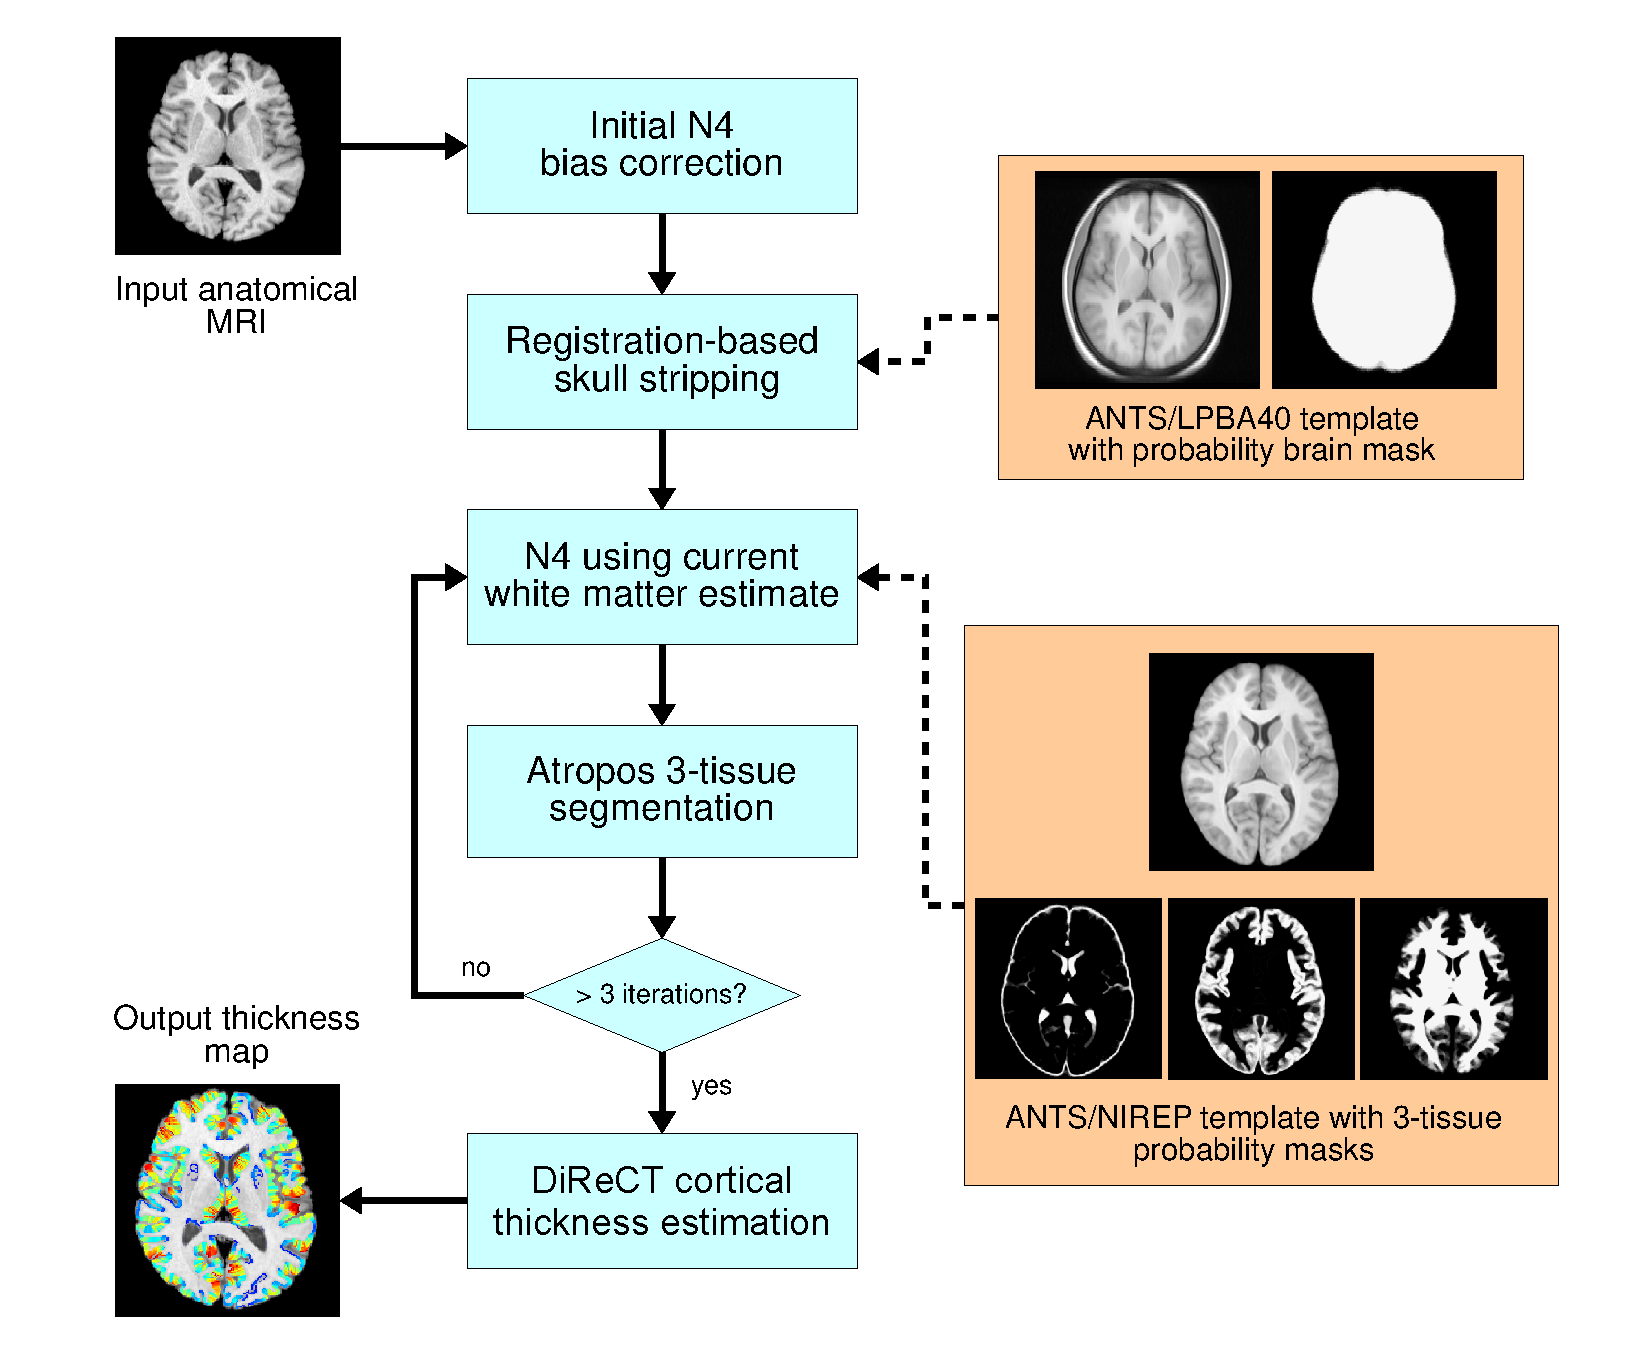
\includegraphics[width=130mm]{Figures/Kapowski_pipeline.pdf}
  \caption{The ANTs T1 processing workflow containing all elements for 
  determining cortical thickness. Not shown is the optional single subject
  to template registration.}
  \label{fig:pipeline}
\end{figure*}

\subsubsection{Anatomical template construction}

Normalizing images to a standard coordinate system
reduces intersubject variability in population studies.  Various
approaches exist for determining the normalized space such as the selection
of a pre-existing template based on a single subject, e.g. the Talairach
atlas \citep{Talairach1988}, or a publicly available averaged group of
subjects, e.g. the MNI \citep{Collins1994} or ICBM \citep{Mazziotta1995}
templates.  Additionally, mean templates constructed from labeled
data can be used to construct spatial priors for improving segmentation
algorithms.
The work of \cite{avants2010} explicitly models the geometric component of the 
normalized space during optimization to produce such mean templates.  Coupling the intrinsic symmetry of 
SyN pairwise registration \citep{avants2011} and an
optimized sharpening/averaging of the template appearance, Symmetric Group
Normalization (SyGN) is a powerful framework for producing optimal population-specific
templates \citep{avants2010} with arbitrary similarity metric choice.  

%One challenge with standard templates is that they may inadvertently bias one's results by enabling better normalization of subjects to which the template is more similar.  This issue is exacerbated when dealing with populations that have high variance (e.g. due to disease) and/or when one's normalization method is low-dimensional (not flexible enough to capture large shape differences). 

%Population-specific templates alleviate some of
%the issues with other template approaches by deriving a most representative image from the population
%\citep{Good2001}.  Large deformation registration algorithms also reduce
%this confound by being less sensitive to the deformation distance
%between subject and target.  Some approaches combine both advantages,
%for instance, the diffeomorphic approach of Joshi et al. employs the
%SSD metric and a shape distance to bring the subject group of images
%into alignment \citep{Joshi2004}.  Variants
%include extension to multiple modalities \citep{Lorenzen2006} and small deformations
%\citep{Geng2009}.  These approaches iteratively minimize group difference in ``congealing''
%towards a representative image template \citep{Learned-Miller2006}.


The ANTs implementation of this technique is currently available as a shell script, 
\verb#buildtemplateparallel.sh#, and a multivariate version,
\verb#antsMultivariateTemplateConstruction.sh#, both of which are distributed as part of
 the ANTs repository.
The latter script permits the construction of multimodal templates (e.g. 
T1-weighted, T2-weighted, and proton density MRI as described in the 
Evaluation section).  Both scripts accommodate a variety of computational resources
for facilitating template construction.  These computational resource possibilities include:
\begin{itemize}
  \item serial processing on a single workstation, 
  \item parallelized processing on a single workstation with multiple cores using \verb#pexec#%
  \footnote{http://www.gnu.org/software/pexec/pexec.1.html},
  \item parallelized processing using Apple's XGrid technology%
  \footnote{https://developer.apple.com/hardwaredrivers/hpc/xgrid\_intro.html}, 
  \item parallelized processing using Sun Grid Engine for cluster-based systems%
  \footnote{http://www.oracle.com/technetwork/oem/grid-engine-166852.html}, and 
  \item parallelized processing using the Portable Batch System for cluster-based systems%
  \footnote{http://www.pbsworks.com/}.
\end{itemize}
Within this work multiple templates were created for all stages of 
image processing and analysis.  The creation of these templates are described
in the corresponding data section.


%Given a set of representative images, 
%$\{I_1, I_2, \ldots, I_M\}$, optimization involves finding the set of paired
%diffeomorphic transformations, $\left\{\left(\phi^1_1, \phi^1_2\right), 
%\left(\phi^2_1, \phi^2_2\right), \ldots, \left(\phi^M_1, \phi^M_2\right) \right\}$,
%the optimal template appearance, $J^*$, and corresponding coordinate system, $\psi(\mathbf{x})$,
%which minimize the following cost function:
%\begin{align}
%  \sum_{m=1}^M \left[
%    D\left( \psi(\mathbf{x}), \phi^m_1(\mathbf{x}, 1) \right) + 
%    \Pi \left( I_m\left(\phi^m_2(\mathbf{x}, 0.5) \right), J^*\left(\phi^m_1(\mathbf{x}, 0.5) \right) \right)
%    \right]
%\end{align}
%where $D$ is the diffeomorphic shape distance, 
%\begin{align}
%  D\left(\phi(\mathbf{x}, 0), \phi(\mathbf{x}, 1)\right) = \int_{0}^1 \| v(\mathbf{x}, t) \|_L dt, 
%\end{align}
%dependent upon the choice of the linear operator, $L$, and
%$v$ is the diffeomorphism-generating velocity field, 
%\begin{align}
%  v\left(\phi(\mathbf{x}, t), t \right) = \frac{d\phi(\mathbf{x}, t)}{dt},\,\,\, \phi(\mathbf{x}, 0) = \mathbf{x}.
%\end{align}
%$\Pi$ is th
%e choice of similarity metric, often cross-correlation \citep{Avants2008a}, calculated in the 
%virtual domain midway between each individual image and the current estimate of the template. 
%
%With initial assignment of $\left\{\left(\phi^m_1, \phi^m_2\right)\right\}$ and $\psi(\mathbf{x})$ 
%to identity, iterative optimization
%involves estimating the pairwise transformations, estimation of the optimal template appearance, and 
%updating $\psi(\mathbf{x})$ by averaging the current estimate of $\left\{\phi_1^m\right\}$.  


\subsubsection{N4 Bias field correction}

Critical to quantitative processing of MRI is the minimization of
field inhomogeneity effects which causes artificial low frequency 
intensity variation across the image.  Large-scale studies, such
as the Alzheimer's Disease Neuroimaging Initiative (ADNI), employ
perhaps the most widely used bias correction algorithm, N3 \cite{sled1998}, 
as part of their standard protocol \citep{boyes2008}.

In \cite{tustison2010}, we introduced an extension of N3, denoted as
N4, which demonstrates improved performance and convergence behavior
on a variety of data.  This improvement is a result of an enhanced 
fitting routine (which includes multi-resolution capabilities) and a modified optimization 
formulation.  For our workflow, the additional possibility of specifying
a weighted mask in N4 permits the use of the current white matter probability map 
calculated during the segmentation pipeline for further improvement of 
bias field estimation.  In addition to its public availability 
through ANTs and the Insight Toolkit, it has also been included in
the popular open source Slicer software package for visualization and medical
image computing \cite{fedorov2011}.

N4 is used in two places during the individual subject processing (cf. Figure
\ref{fig:pipeline}).  Following conversion of the raw dicom T1-weighted image
to Nifti format using our related \verb#Neuropipedream# set of raw image conversion
and organization tools%
\footnote{
http://sourceforge.net/projects/neuropipedream/
}, N4 is used to generate an initial bias corrected image for use in
brain extraction.  The input mask is created by adaptively thresholding 
the background from the foreground using Otsu's algorithm \cite{otsu1979}.
Following brain extraction, the three-tissue segmentation involves iterating
between bias field correction using the current white matter posterior 
probability as a weight mask and then using that bias corrected image
as input to the Atropos segmentation step (described in subsequent sections). 

\subsubsection{Atropos 3-tissue segmentation}

In \cite{avants2011a} we presented an open source $n$-tissue segmentation software tool
(which we denote as ``Atropos'') attempting to distill 20+ years of active research in this area
particularly some of its most seminal work (e.g. \cite{zhang2001,ashburner2005}). 
Specification of prior probabilities includes spatially varying Markov Random Field modeling, 
prior label maps, and prior probability maps typically derived from our template building 
process.  Additional
capabilities include handling of multivariate data, 
partial volume modeling \cite{shattuck2001}, a memory-minimization mode,
label propagation, a plug-n-play architecture for incorporation of novel likelihood models
which includes both parametric and non-parametric models for both scalar and tensorial
images, and alternative posterior formulations for different segmentation tasks.

\subsubsection{Brain extraction}

Brain extraction using ANTs combines template building, high-performance
brain image registration \citep{avants2011}, and Atropos with topological refinements.  
An optimal template for brain extraction is 
generated offline using labeled brain data.  For example, in this work we use the LPBA40 data 
for generating a brain extraction template and a corresponding brain probability mask which is
available on the website associated with this submission. 

  The warped template probability map is thresholded at 0.5 and the resulting mask is dilated
with a radius of 2.  Atropos is used to generate an initial 3-tissue segmentation estimate within the mask
region.  Each of the three tissue masks undergo specific morphological operations which are then
combined to create a brain extraction mask for use in the rest of the cortical thickness workflow.

A comparison using open access brain data with publicly available brain extraction algorithms 
including  AFNI's \verb#3dIntracranial# \citep{ward1999}, FSL's \verb#BET2# \citep{smith2002}, 
Freesurfer's \verb#mri_watershed# \citep{segonne2004}, and BrainSuite \citep{dogdas2005}  demonstrated
that our combined registration/segmentation approach \citep{avants2010a} performs at the top level
alongside BrainSuite (tuned) and FreeSurfer.


\subsubsection{DiReCT Cortical Thickness Estimation}

Although the basic formulation of DiReCT as reported in this work is as it 
was introduced in \cite{das2009}, we have made several 
improvements (perhaps the most significant being that this particular 
ITK-compatible implementation has been significantly multi-threaded,
is written in ITK coding style, and has been made publicly available through 
ANTs complete with a unique user interface design developed specifically for 
ANTs tools.  

\subsection{Public Data Resources}

\subsubsection{LPBA40 Data for Skull Stripping}

For the brain extraction step
we used the data from the LPBA40 repository \citep{shattuck2008}.
These data consist of 40 high-resolution 3D Spoiled Gradient Echo
(SPGR) MRI acquisitions which were manually labeled delineating
56 brain structures.  Additional post processing 
included automated brain extraction using FSL's brain extraction tool 
\citep{smith2002} which was followed by manual corrections.  These
40 brain masks are also included with the database.  

All 40 subjects were used to create a population-specific
unbiased average template \cite{avants2010}.  The brain masks corresponding 
to the 20 subjects were warped to the template space using the 
transforms derived during the template building process.  A template 
probability mask was created by averaging the warped brain masks.
For brain extraction of any single individual this ANTS-based LPBA40 template 
is coarsely registered to the single subject brain.  The template
probability brain mask is warped to the individual subject and 
is used as the initial brain mask estimate.  As mentioned previously,
Atropos and binary morphological operations are used to refine the
brain mask estimate.

\subsubsection{NIREP Data for 3-Tissue Segmentation}

The nonrigid image registration evaluation project is an ongoing 
framework for evaluating image registration algorithms \citep{christensen2006}.
The initial data set introduced into the project consists of 
16 (8 male and 8 female) high resolution skull-stripped brain 
data with 32 cortical labels manually drawn using published protocol.
Given the gray matter labels, the white matter and CSF were identified 
for each of the 16 subjects using Atropos.  Similar to the LPBA40
data set, a NIREP template was created from all 16 subjects and each the
warped labels were used to create probabilistic estimates of the 
labeled region boundaries. These probability maps were used as 
spatial prior probabilities during the 3-tissue segmentation component
of the pipeline.  Using SyN, the NIREP template is registered to the
extracted individual subject brain which is followed by a warping of the 
NIREP priors to the space of the individual subject.  The initial warped 
white matter probability map is used as the weighted confidence mask 
in the follow-up bias correction step.

\subsection{IXI Data for Pipeline Evaluation}

The IXI data%
\footnote{
http://biomedic.doc.ic.ac.uk/brain-development/
}
consists of approximately 600 healthy subjects imaged at three sites 
using several modalities (T1-weighted, T2-weighted, proton density, magnetic 
resonance angiography, and diffusion tensor imaging).  The 
database also consists of  demographic information such as age, weight,
height, ethnicity, occupation category, educational level, and marital status.
The number of subjects spanning a range of demographic characteristics makes
this a rich data set for validating and exploring correlations with cortical 
thickness measured using the ANTs pipeline.

\begin{figure}
  \centering
  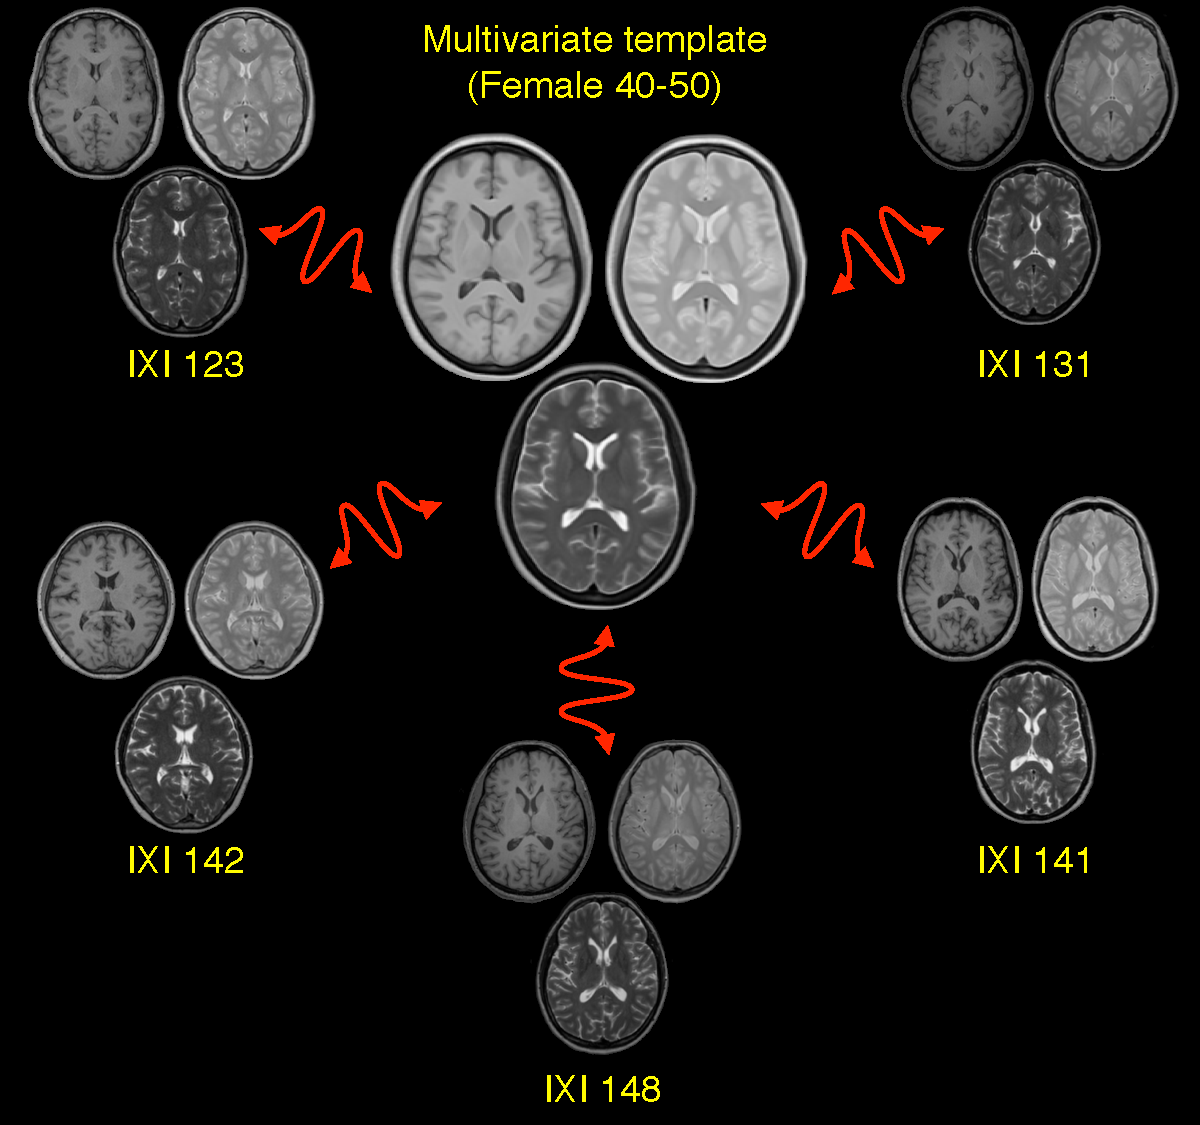
\includegraphics[width=90mm]{Figures/template.pdf}
  \caption{Sample multivariate template constructed from a subset of the IXI data (female, age 40--50).  Axial slices of five of the 37 total subjects from this cohort are shown. }
  \label{fig:template}
\end{figure}



\section{Introduction}

%% References with bibTeX database:

%\section*{Acknowledgments}


\section{Notes/Thoughts}
\begin{itemize}
  \item Several kinds of bias have cropped up in the neuroimaging
  community recently:
  \begin{itemize}
    \item{methodological bias}:  Kreikesgorte
    \item{statistical bias}:  Vul2009, Tustison2012
    \item  What about the dead salmon fmri study---multiple comparisons correction?
    \item The single subject VBM study (assuming the single subject is representative of the population).
    \item{overview}:  9 circles of scientific hell ---neuroskeptic %http://blogs.discovermagazine.com/neuroskeptic/?p=1205#.UYZxyJWO7Tx
    \item Types of measurement bias: \cite{sackett1979}
    \begin{itemize}
      \item Instrument bias (code as a type of instrument which needs to be calibrated correctly).
      \item Expectation bias (i.e. confirmation bias)
    \end{itemize}  
  \end{itemize}
  We are concerned with the latter two.
  \item How does one avoid confirmation bias?  If I'm comparing my
  algorithm to somebody else's algorithm, I'm going to be naturally
  predisposed to confirmatory evidence that my algorithm is better
  while neglecting (most likely not with intent of doing so) evidence
  that disconfirms my original belief (that my algorithm is better).
  Richard Feynman quote (Cargo Cult Science):  
  \begin{quote} 
  The first principle [of science] is that you must not fool yourself�--and you are the easiest person to fool. So you have to be very careful about that. After you've not fooled yourself, it's easy not to fool other scientists. You just have to be honest in a conventional way after that.
  \end{quote}
  \item One particular aspect of the previous item is that it needs 
  to be highlighted if somebody codes up the algorithm
  to be compared themselves.  Writing bug-free code is difficult.  Look
  at how many bug fixes are provided by the ITK community on a daily
  basis.  
  \item Also, is simply saying that one algorithm is better than 
  another sufficient?  Should there be some theoretical explanation
  for it.  For example, when I wrote my DMFFD image registration paper,
  the comparison wasn't IRTK vs. DMFFD but rather FFD vs. DMFFD and
  there were theoretical reasons why performance should be better
  with the latter.  Also, I insisted to the reviewer on not using IRTK 
  for comparison since there are also so many other performance-related
  issues (type of interpolation, gradient step, metric, metric implementation, etc.) which would confound
  comparisons.  Also, it probably helped that the theme had a more specific,
  more verifiable focus, i.e. DMFFD produces a more efficient energy minimizer
  since it acts as a preconditioner in the standard gradient descent
  optimization.
  \item Comparisons are best made with publicly available data and
  results of the comparisons should be made available.
  \item Operating system needs to be defined.  Freesurfer results
  varied with MacOSx.
  \item Ideally, the authors of the new algorithm would work
  with the authors of the compared algorithm.  Given human
  nature, this type of cooperation is not guaranteed.  However,
  a minimum set of information is needed.
  \item Arno Klein as an example of somebody who did it right.  Takes a
  lot of work.
  \item 
  \item The source of the package software needs to be defined.  For 
  example, N4 has been
  instantiated in Slicer, ANTs, and c3d (also might be implemented
  in one of Styner's NITRC projects).  However, each might use
  different default parameters and have other tweaks which effects
  performance.  In Vladimir Fonov's github repository containing 
  various processing scripts for MINC, one can see from the history
  how N4 was used but then the users switched back to N3MNI (due to 
  performance issues?).  However, they used N4 out of the c3d package
  which the original authors (N.T./B.A.) haven't touched in three years
  so the parameters aren't optimal (shrink factors = 4, spline distance
  = 100 with 3 levels: $100\times50\times50$).  Changing these parameters 
  (which are crucial to performance) isn't
  accessible to the user from c3d.  
  \item Great resources for code-sharing
  	\begin{itemize}
		  \item github
		  \item NITRC
		  \item ITK
		\end{itemize}
\end{itemize}

\section*{References}

\bibliographystyle{elsarticle-harv}
\bibliography{references}


%% Authors are advised to submit their bibtex database files. They are
%% requested to list a bibtex style file in the manuscript if they do
%% not want to use model1-num-names.bst.

%% References without bibTeX database:

% \begin{thebibliography}{00}

%% \bibitem must have the following form:
%%   \bibitem{key}...
%%

% \bibitem{}

% \end{thebibliography}


\end{document}

%%
%% End of file `elsarticle-template-1-num.tex'.
